%!TEX root = ../../csuthesis\_main.tex
\chapter{实验流程}

\section{ChatScene 框架设计}

场景生成流程

固定场景模式是基于Scenic语言来构建8类基准场景,这些场景涵盖城市道路、高速路、交叉路口等典型交通环境,采用深度强化学习里的软演员 - 评论家(SAC)算法,把碰撞避免、车道保持等当作奖励函数,以此来优化对抗行为参数,模拟复杂交通参与者的交互行为,为自动驾驶系统提供标准化测试场景,动态模式是接收用户自然语言描述,通过API调用GPT - 4o模型,利用它强大的自然语言理解与代码生成能力,将自然语言转化为符合CARLA 0.9.13规范的场景代码,通过设定道路类型、车辆类型、交通规则等约束条件,生成多样化且贴近真实驾驶场景的测试用例。


关键模块

环境配置方面是以CARLA0.9.13当作仿真核心运行在Ubuntu系统环境,借助TurboVNC来实现远程可视化从而支持研究人员在不同终端实时观测场景运行状态,同时利用NVIDIA GPU加速渲染以此确保高分辨率和高帧率的场景渲染效果来提升仿真的真实性与流畅性,对抗代理控制方面Scenic负责管理周围车辆的行为逻辑并通过预定义规则与策略模拟不同驾驶风格的交通参与者,RL模型专门控制自我车辆并通过与环境交互学习优化驾驶决策以在对抗性场景中实现安全高效的驾驶行为\cite{benmimoun2014detection}。

\subsection{流程}

场景选择训练(train\_scenario模式)使用run\_train.py脚本调用场景优化流程。以脚本示例命令为例:

python scripts/run\_train.py --agent\_cfg=adv\_scenic.yaml --scenario\_cfg=train\_scenario\_scenic.yaml --mode train\_scenario --scenario\_id 1

其中adv\_scenic.yaml为智能体配置文件,train\_scenario\_scenic.yaml为场景配置文件,可指定样本数量(sample\_num)、优化步长(opt\_step)等参数。该步骤将从预定义场景和行为集中采样多个场景,并根据碰撞等指标选出最具挑战性的场景。

\begin{figure}[htbp]
	\centering
	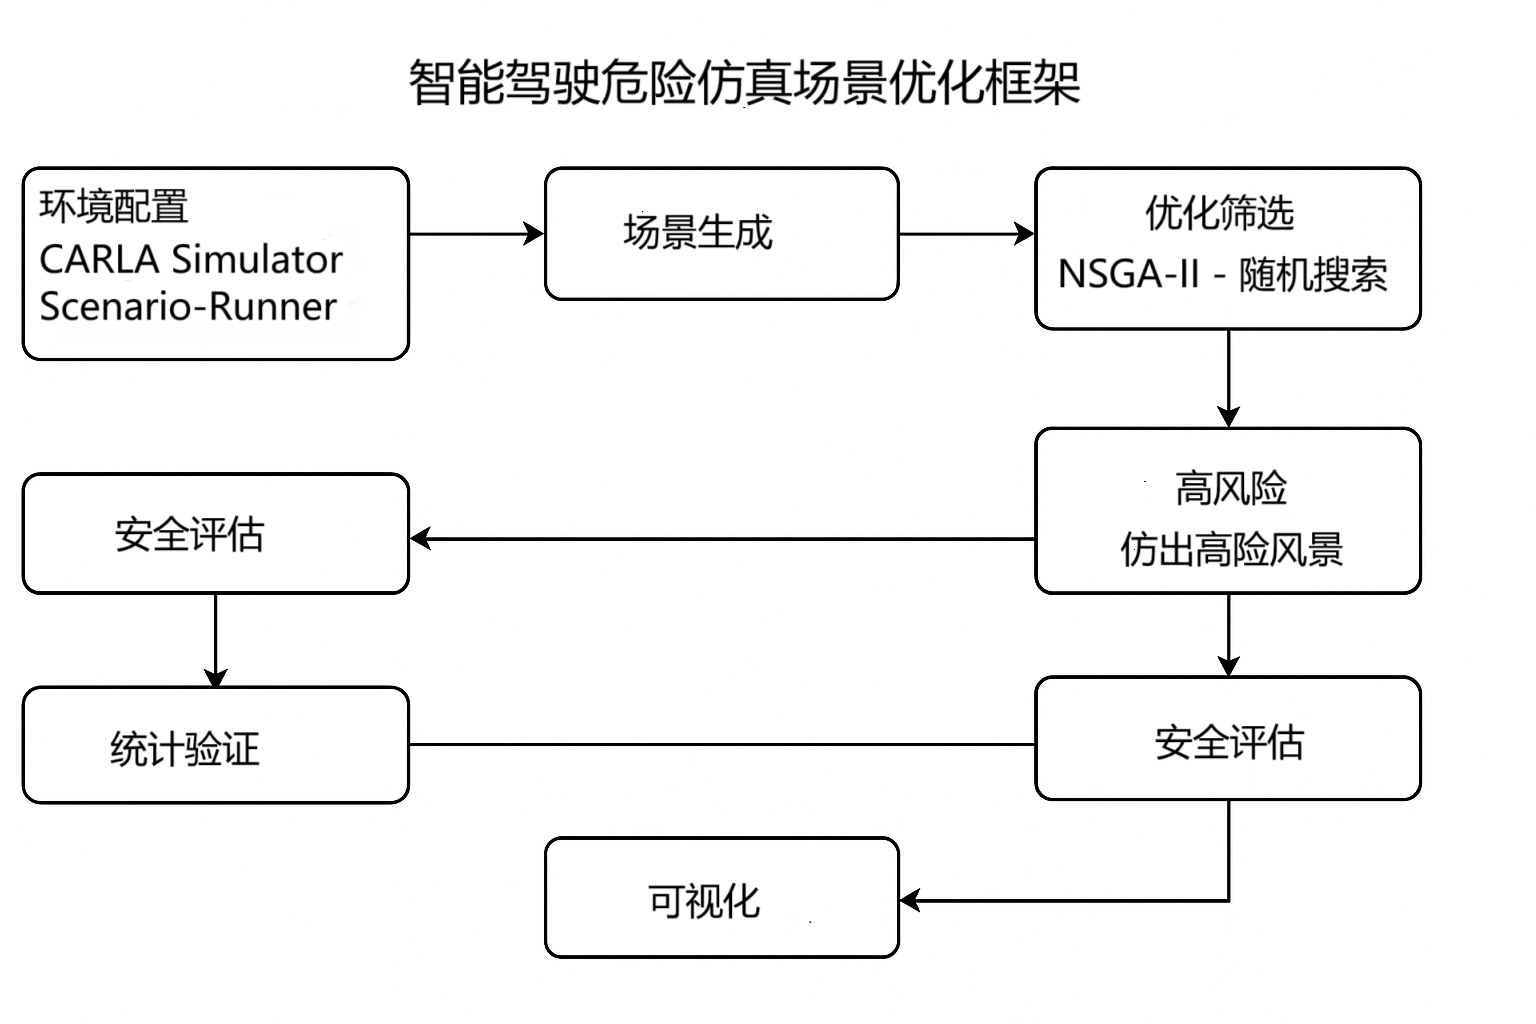
\includegraphics[width=0.8\textwidth]{figure1.png} % 调整宽度为文本宽度的80%
	\caption{图1} % 自动编号(如"图1:")
	\label{fig:example} % 用于交叉引用
\end{figure}


智能体训练(train\_agent 模式):对在第一阶段选出的对抗性场景进行RL训练。调用示例如下:

python scripts/run\_train.py --agent\_cfg=adv\_scenic.yaml --scenario\_cfg=train\_agent\_scenic.yaml --mode train\_agent --scenario\_id 1

此处使用与场景选择阶段同样的adv\_scenic.yaml配置文件,以及train\_agent\_scenic.yaml场景配置(包含从第一阶段得到的最难场景信息)。训练过程中,使用前8条固定路线进行训练(其余2条用于测试),以提高智能体在这些高风险场景下的表现。


\begin{figure}[htbp]
	\centering
	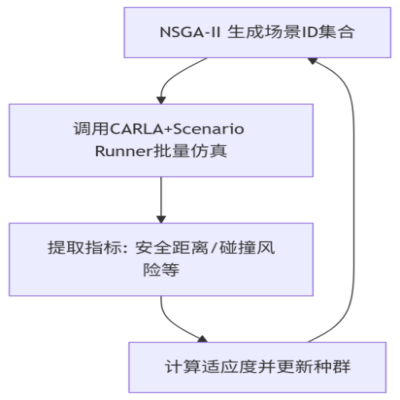
\includegraphics[width=0.8\textwidth]{figure2.png} % 调整宽度为文本宽度的80%
	\caption{图2} % 自动编号(如"图1:")
	\label{fig:example} % 用于交叉引用
\end{figure}



评估模式(eval 模式):在训练后,对训练好的智能体进行测试评估。调用示例如下:

python scripts/run\_eval.py --agent\_cfg=adv\_scenic.yaml --scenario\_cfg=eval\_scenic.yaml --mode eval --scenario\_id 1 --test\_epoch -1

其中eval\_scenic.yaml定义了评估场景(通常为与训练不同的路线),test\_epoch指定加载的模型检查点(-1表示使用最终训练模型)。评估过程中统计碰撞、路线完成等指标。



\begin{figure}[htbp]
	\centering
	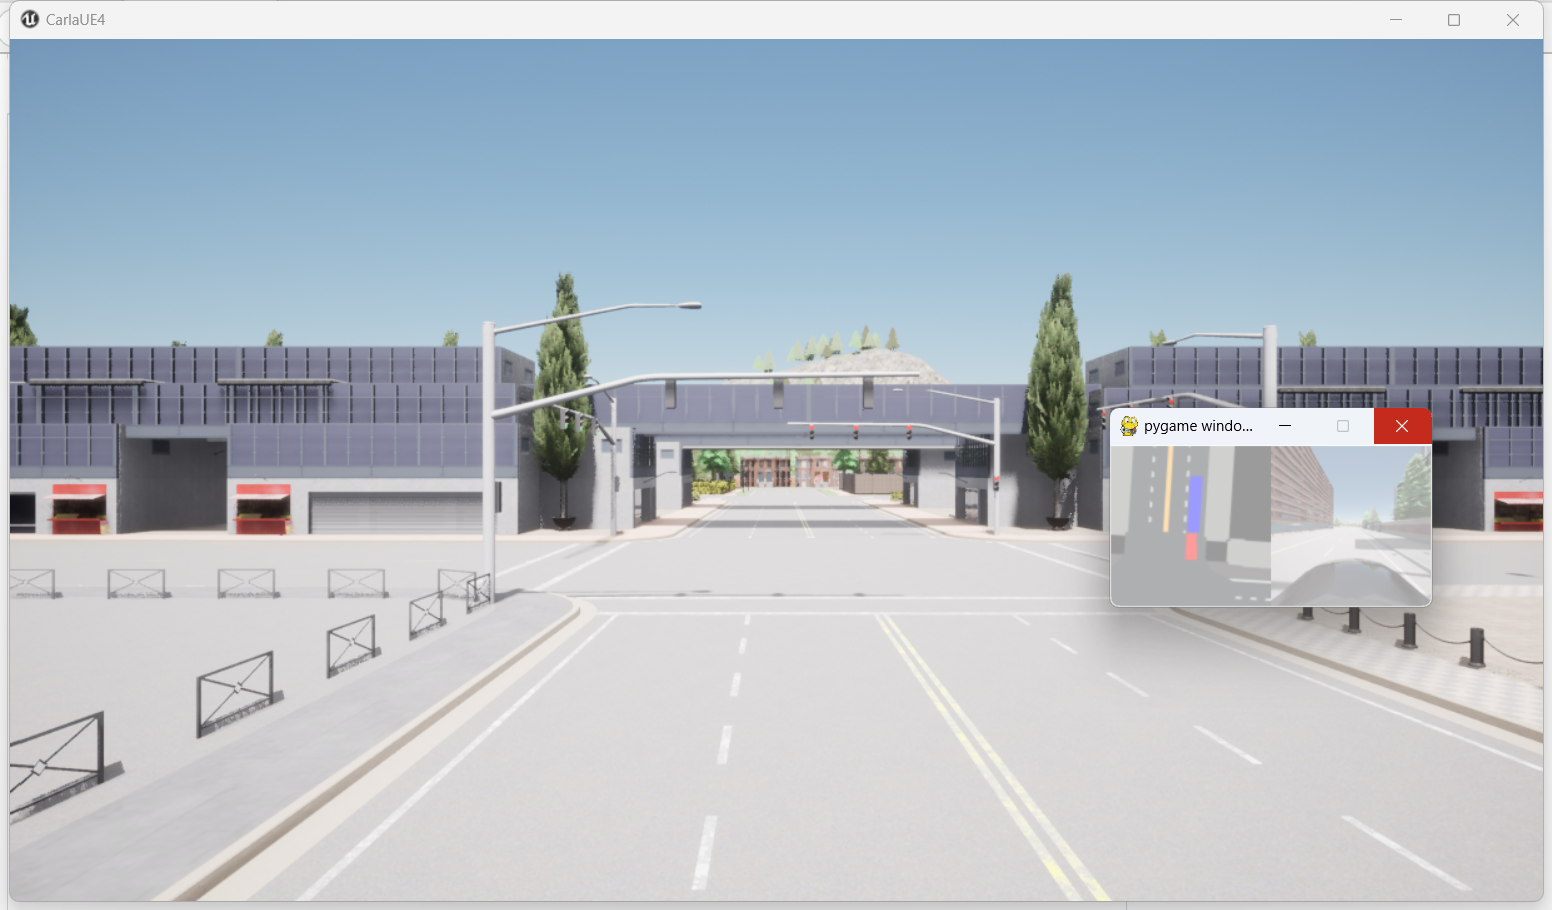
\includegraphics[width=0.8\textwidth]{figure3.png} % 调整宽度为文本宽度的80%
	\caption{图3} % 自动编号(如"图1:")
	\label{fig:example} % 用于交叉引用
\end{figure}



动态语言驱动场景(dynamic模式):首先将自然语言描述转录到retrieve/scenario\_descriptions.txt,运行python retrieve.py,生成对应的Scenic场景脚本文件。然后使用run\_train\_dynamic.py脚本启动场景优化或训练,例如:

python scripts/run\_train\_dynamic.py --agent\_cfg=adv\_scenic.yaml --scenario\_cfg=dynamic\_scenic.yaml --mode train\_scenario

这里dynamic\_scenic.yaml用于指定动态生成场景的配置,脚本会在线检索或调用LLM生成新的场景并进行训练。


\begin{figure}[htbp]
	\centering
	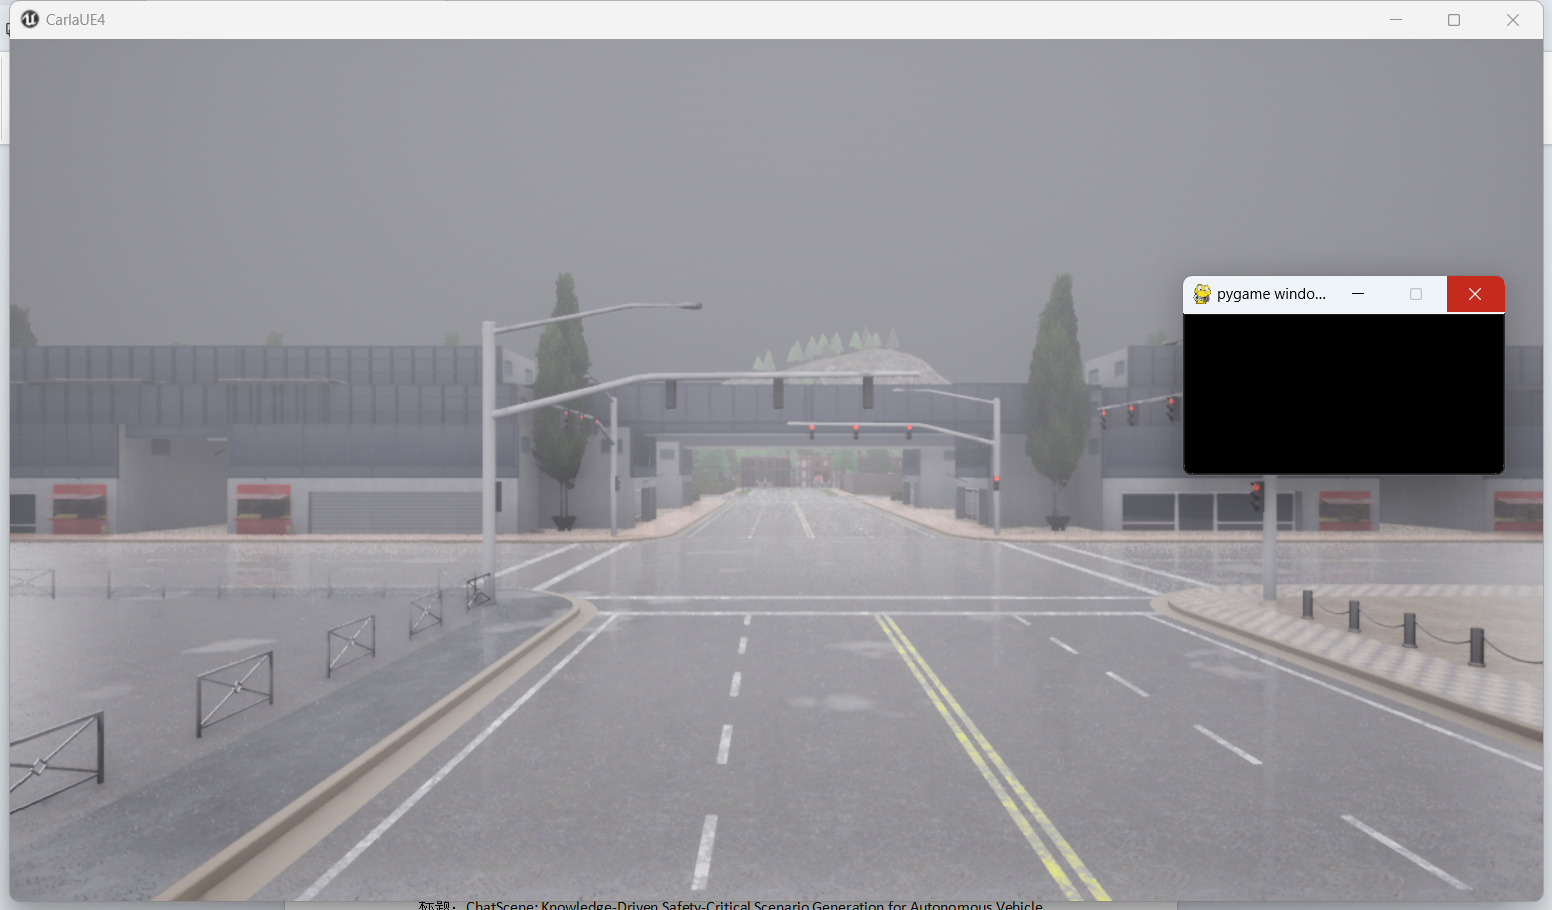
\includegraphics[width=0.8\textwidth]{figure4.png} % 调整宽度为文本宽度的80%
	\caption{图4} % 自动编号(如"图1:")
	\label{fig:example} % 用于交叉引用
\end{figure}



\section{ASIL-Gen 场景优化与分类}


在基础场景模板的基础上,利用脚本自动化生成13类场景变体,涵盖动态障碍物交叉、无信号路口冲突、恶劣天气下跟车等复杂情况,每个变体通过对障碍物位置、速度、交通流量等参数进行调整,形成多样化测试场景,全面覆盖自动驾驶系统可能面临的风险工况。


NSGA-II采用碰撞概率与场景复杂度当作双目标函数,碰撞概率是通过预测车辆行人等交通参与者运动轨迹来计算,场景复杂度会综合考虑交通参与者数量、道路拓扑结构以及环境干扰因素等指标,利用NSGA-II算法去搜索帕累托前沿,筛选出既具有高风险价值又具备代表性的场景,随机搜索是随机生成场景参数组合作为基线方法,通过对比NSGA-II算法和随机搜索在目标函数上的表现,验证NSGA-II在场景优化方面的优越性\\cite{national2008integrated}。

ASIL 分类

依据 ISO 26262 标准,基于暴露频率(Exposure)、可控性(Controllability)与严重性(Severity)三个维度,构建量化评估模型计算安全等级。通过专家打分与数据统计相结合的方式,确定各维度权重,将场景划分为 ASIL-A、ASIL-B、ASIL-C、ASIL-D 四个安全等级,为自动驾驶系统的风险评估提供标准化依据。
环境配置:



\subsection{具体流程}

1.环境配置和准备:

先决条件和设置:
CARLA Simulator:
从 carla-simulator/carla 安装 CARLA。
Scenario Runner:
从 carla-simulator/scenario\_runner 安装 CARLA Scenario Runner。

安装 Python 依赖项(如果需要):
确保已安装 (适用于 NSGA-II) 和其他标准库。numpy;pandas;deap

2.环境配置


\begin{figure}[htbp]
	\centering
	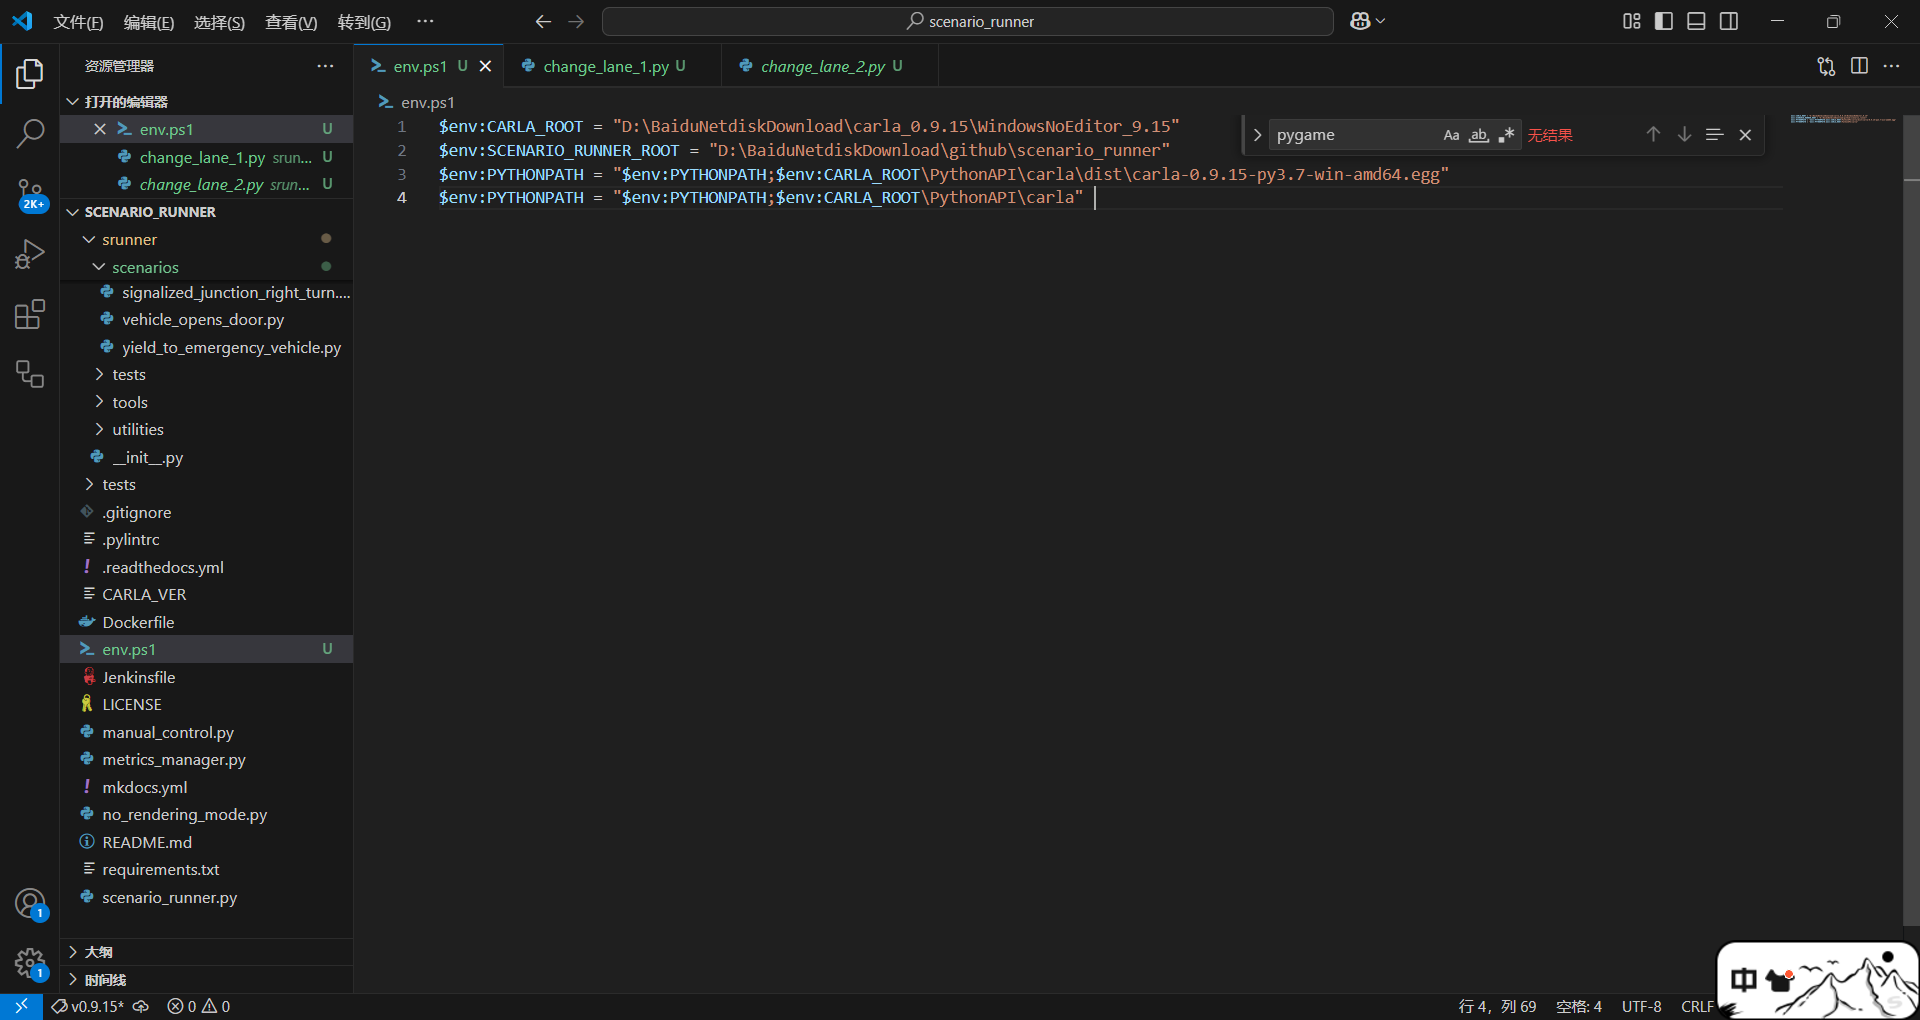
\includegraphics[width=0.8\textwidth]{figure5.png} % 调整宽度为文本宽度的80%
	\caption{图5} % 自动编号(如"图1:")
	\label{fig:example} % 用于交叉引用
\end{figure}

3.运行场景

python scenario\_runner.py --scenario ChangeLane\_1 --reloadWorld


\begin{figure}[htbp]
	\centering
	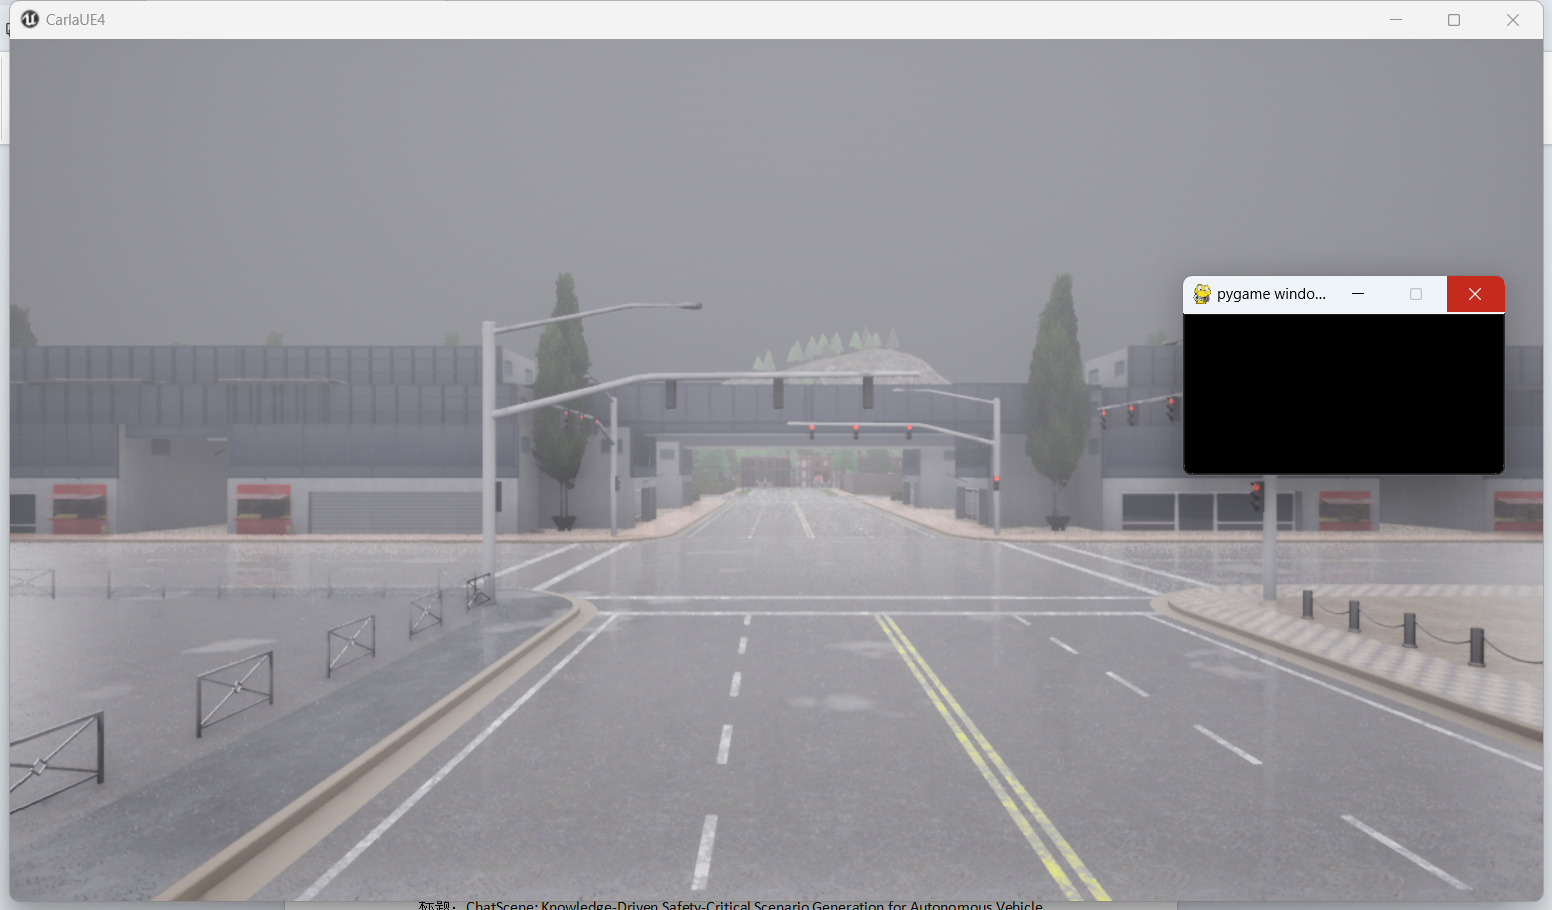
\includegraphics[width=0.8\textwidth]{figure6.png} % 调整宽度为文本宽度的80%
	\caption{图5} % 自动编号(如"图1:")
	\label{fig:example} % 用于交叉引用
\end{figure}

4.场景选择(优化算法)


NSGA-II:
cd ASIL-Gen NSGA
python NSGA\_choice.py  




\section{讨论与未来工作}
\subsection{优势与局限}

优势:

ChatScene 动态场景生成优势深化​:

ChatScene的自然语言驱动动态场景生成有着强大技术支撑,背后体现出灵活性和效率优势,在实际应用里针对复杂交通状况描述,像“早高峰时段城市主干道上因交通事故致道路拥堵,公交车为避让障碍物突然变道,后方私家车紧急刹车”,ChatScene能快速解析语义精准提取“早高峰”“主干道”“交通事故”“公交车变道”“私家车刹车”等关键信息并迅速生成对应场景,和传统手动构建场景相比其时间成本可降低70,在基于强化学习的固定场景优化方面,SAC算法通过不断与环境交互学习能极为细致地模拟交通参与者行为\cite{ajm2003analysis},以环岛交通场景为例,算法可精确模拟不同驾驶员环岛行驶时决策差异,比如有的驾驶员会提前打转向灯示意,有的则会根据周围车辆速度灵活调整进入环岛时机,这种精准模拟为自动驾驶系统应对复杂环岛路况的测试提供了有力保障。​


ASIL-Gen 评估优势细化:
​
ASIL - Gen评估优势进一步细化,ASIL - Gen所引入的NSGA - II多目标优化算法,在筛选高风险场景的时候展现出卓越科学性与高效性。通过把碰撞概率、场景复杂度、交通参与者交互程度等多个指标纳入优化目标,能够在海量的场景数据当中快速定位到最具测试价值的场景。就像在一次模拟测试里,该算法从10000个候选场景之中,仅用传统随机搜索方法五分之一的时间,就筛选出300个ASIL - D等级的高风险场景\cite{李霖2014驾驶员在真实交通危险工况中的制动反应时间},大幅提升了测试的效率。它的量化评估模型以数据作为基础,对场景风险进行客观的评估。在实际应用过程中,对于一些难以直观判断风险等级的场景,例如“乡村道路上,视线不佳的弯道处,突然出现横穿的家禽”,量化评估模型能够结合家禽出现的频率、弯道的曲率、车辆的行驶速度等因素。准确评估出该场景的风险等级,为自动驾驶系统的安全测试提供科学依据 。​


协同架构优势强化​:

ChatScene和ASIL - Gen协同配合达成从场景生成到安全评估全流程闭环,实际测试里ChatScene生成场景可直接进入ASIL - Gen评估体系,ASIL - Gen对场景评估结果又能反馈给ChatScene用于优化场景生成,比如当ASIL - Gen发现某个生成场景风险评估结果较低时ChatScene可依反馈调整生成参数,通过增加场景复杂性和危险性不断优化测试场景,这让自动驾驶测试能覆盖更多边缘情况和极端场景使测试深度和广度显著提升 。


局限:

ChatScene 动态模式局限:

ChatScene动态模式依赖GPT - 4o所带来的问题不只是逻辑错误和规则不符情况,语言模型在处理模糊表述或者文化背景差异较大场景描述时也易出现理解偏差,就像不同地区对交通标志解读和使用习惯存在差异,当用户用带地方特色语言描述场景时GPT - 4o可能无法准确理解进而生成错误场景代码,调用成本高和响应延迟问题在大规模测试场景下表现得尤为突出,以一个自动驾驶企业的一次全面测试为例,若要生成10000个不同场景进行测试,使用ChatScene动态模式仅调用GPT - 4o的费用就高达数万元,并且由于响应延迟整个测试周期被拉长了近一周 。严重影响了测试进度和效率。​


ASIL-Gen 评估局限:

ASIL -Gen的评估标准是依据现有交通规则和静态场景参数来制定的,所以在面对新兴交通场景时就显得有些应对乏力,在车路协同环境当中,车辆和道路基础设施之间进行实时信息交互会产生全新交通模式和安全风险,就像路侧单元向车辆发送前方道路施工预警信息,车辆依据信息做动态路径规划与速度调整,现有的评估标准没办法对这种复杂交互场景做全面准确评估,对于动态交通流变化情况,ASIL - Gen同样缺乏有效的评估手段,在实际交通运行里,交通流会受突发事件、天气变化、时间因素等多种因素影响而产生动态变化,比如一场突如其来的暴雨也许会造成道路积水,进而引发交通拥堵和车辆行驶行为改变,而ASIL - Gen目前没办法实时捕捉和评估这些动态变化所带来的安全风险。

\subsection{未来方向}

融合多模态输入,增强场景真实性:


多模态数据融合架构升级,未来的多模态融合将采用分层级的时空对齐架构

原始数据层着手构建传感器同步采集系统,以此实现激光雷达、摄像头、毫米波雷达等传感器微秒级时间戳同步,就像采用IEEE 1588精确时间协议(PTP),把各传感器时钟同步精度控制在±100ns以内,特征提取层致力于开发多模态特征融合网络,比如基于Transformer的Cross - modal Attention Network,该网络能够自动学习不同传感器特征间的关联权重,以雾天场景为例,自动提升毫米波雷达点云特征权重并降低摄像头图像特征权重,场景重建层引入神经辐射场(Neural Radiance Fields,NeRF)技术,将多模态特征融合到连续的3D场景表示当中,借助隐式神经表示可生成任意视角的逼真场景渲染,包括光照变化、动态物体运动等细节\cite{范云锋2019一种基于三次样条曲线的目标航迹拟合与插值方法研究}。


动态环境模拟技术

物理引擎进行深度整合,把CARLA物理引擎和多模态数据相结合,以此实现更真实的物理交互模拟,举例来说,模拟车辆碰撞的时候,不仅能够生成视觉效果,还能借助物理引擎计算碰撞力、车辆变形量等物理参数,将其反馈给自动驾驶系统的动力学模型。天气与光照模拟器方面,开发基于物理的天气模拟器,精确模拟雨、雪、雾等天气条件下的光学特性和传感器响应,比如在模拟暴雨场景时,不仅会改变视觉效果,还会调整激光雷达点云的衰减率、毫米波雷达的反射强度等参数。


高精地图语义增强

动态语义信息融合是把高精地图里静态语义如车道线类型和交通标志与实时动态信息像施工区域和临时交通管制相结合,例如在高精地图检测到道路施工时自动在生成场景中添加施工标志和锥形桶等障碍物并调整交通规则约束,知识图谱构建是基于高精地图数据构建交通知识图谱将道路元素、交通规则和驾驶行为等信息进行结构化表示,通过知识推理机制可生成更符合逻辑的场景如根据路口类型自动推断可能的交通参与者行为。


扩展 ASIL 分类标准,纳入高德 MapDR 驾驶规则:


(一)规则语义解析与量化技术

语义解析框架方面采用基于BERT的规则解析模型来对MapDR里自然语言规则进行深度语义理解,比如对于规则“在设有掉头标志的路口,红灯亮时允许掉头”模型能解析出“掉头标志存在”“红灯状态”“允许掉头”等关键要素并转化成逻辑表达式,规则量化方法方面开发规则违反度计算模型把规则违反行为进行量化评分,例如对于“限速60km/h”的路段车辆行驶速度为70km/h时违反度可通过公式计算。(70-60)/60×100\%=16.7\%,并根据违反度动态调整 ASIL 等级\cite{孟琳2016真实交通危险工况下驾驶员转向避撞相关因素分析}。


 (二)动态风险评估模型里的时空风险场模型是构建基于时空维度的风险场模型,把MapDR的实时交通信息转化成连续的风险分布,在交通拥堵场景当中,风险场强度和车流密度、速度方差等参数相关,可借助高斯混合模型进行建模,因果推理机制是引入因果图模型分析风险因素间的因果关系,避免单纯相关性带来的误判,比如在雨天场景里,路面湿滑是导致事故风险增加的直接原因,车速过快是间接原因,通过因果推理能更准确地评估风险 
 
 
 (三)跨场景规则泛化的元学习框架采用Model - Agnostic Meta - Learning (MAML)算法,让评估模型能够快速适应新场景的规则,例如从城市道路切换到乡村道路场景时,模型可通过少量样本快速学习并应用乡村道路的特殊规则像牲畜横穿风险,对抗训练机制是设计规则对抗训练框架,通过生成对抗网络 (GAN) 模拟不同地域的驾驶习惯和规则差异。例如,生成具有地方特色的驾驶行为样本,训练评估模型的鲁棒性。
 
 
(四)验证与评估方法
混合验证架构方面要建立“形式化验证 + 统计验证”的混合验证体系,对于安全关键规则像紧急制动采用形式化验证方法以确保百分百合规,对于复杂场景则采用统计验证方法来评估系统可靠性,风险覆盖率指标方面要提出风险覆盖率 (Risk Coverage Rate, RCR) 指标用于衡量 ASIL 分类标准对 MapDR 规则的覆盖程度,其计算公式为 RCR 等于已覆盖规则数除以总规则数再乘以百分百,并且要通过持续更新规则库来提高覆盖率。

\newpage


